\section{MAGIC Intro}%
\label{sec:magic}
\begin{wrapfigure}{r}{0.4\textwidth}
		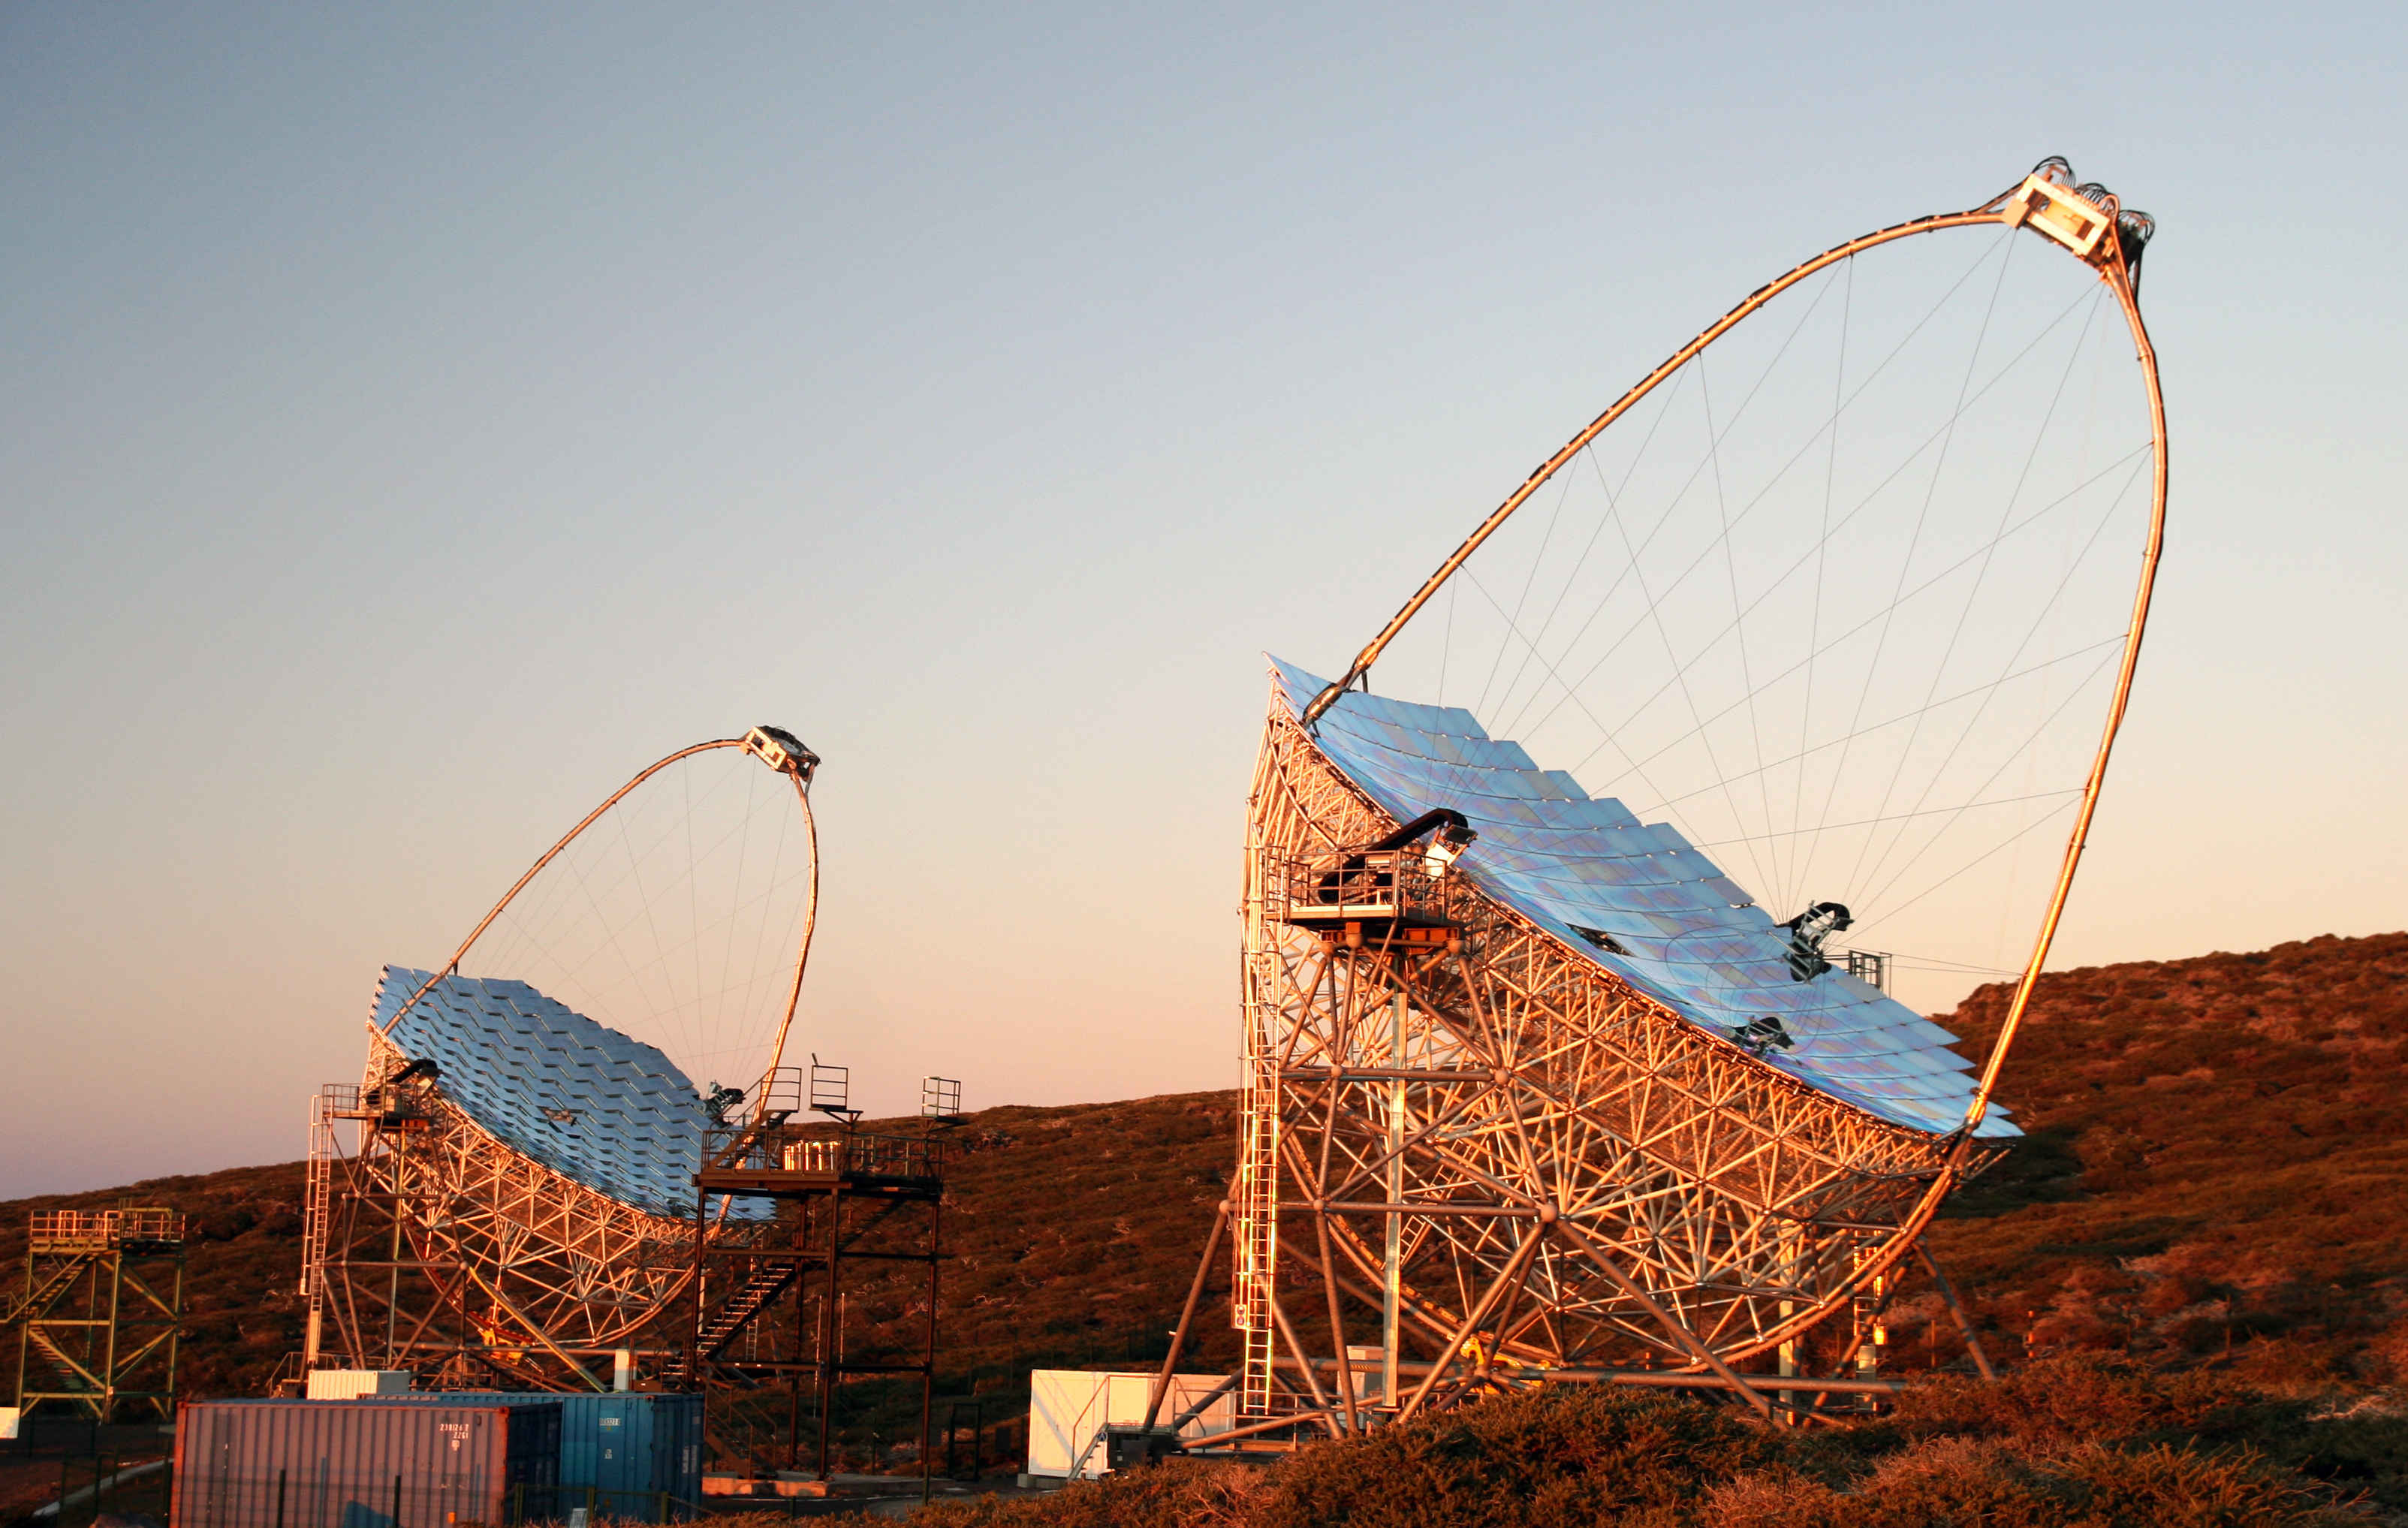
\includegraphics[width=\linewidth]{pictures/magic.JPG}
		\caption{pi}
		\label{fig:pi}
\end{wrapfigure}
Magic ist derzeit (16.11.2016) das größte Stereoteleskop mit dem die
Detektion von Tscherenkov-Schauern in einem Energiebereich von
\SIrange{0}{10}{\electronvolt} möglich ist.
Es steht auf der Insel La Palma auf einer Höhe von \SI{10}{\meter}.

Trifft ein Teilchen mit Überlichtgeschwindigkeit in einem Medium, so emittiert
dieses einen Tscherenkov-Kegel. 
Die ultrarelativistischen Teilchen welche auf die Erdatmosphäre treffen
Wechselwirken mit den darin enthaltenen Teilchen beispielsweise über
Bremsstrahlung, Paarerzeugung \ldots und produzieren somit weitere
relativistische Teilchen welche wiederum Tscherenkov kegel erzeugen.
Die dadurch erzeugten Lichtblitze können durch Tscherenkov-Teleskope detektiert
werden.
Die Spiegelfläche von \SI{10000}{\meter\squared} besteht aus \num{100} einzelnen
Spiegeln welche in der wtf-Formation angeordnet sind und auf \num{1000}
Photomultiplier mit einem Field of View von \SI{90}{\degree} abbilden. 


Sensitivitätsbereich

\begin{itemize}
  \item Teleskop
  \item Datenanalyse
\end{itemize}

\begin{itemize}
  \item Tscherenkov-Schauer
  \item Welche Plots sagen was aus?
    \begin{itemize}
      \item SED, $\theta^2$, Lichtkurve
    \end{itemize}
\end{itemize}

\clearpage
